% ===========================================================================
%  PÔSTER / BANNER CIENTÍFICO — SIC 2026
%  XIII Seminário de Iniciação Científica do IFNMG — Campus Januária
%
%  Formato    : A0 retrato (841 × 1189 mm)
%  Classe     : a0poster
%  Colunas    : paracol (texto corrido, sem blocos rígidos)
%  Compilação : pdflatex → pdflatex
%
%  ► INSTRUÇÕES AO ALUNO:
%    - Substitua todo texto entre [COLCHETES] pelo seu conteúdo.
%    - Não altere o preâmbulo (antes de \begin{document}).
%    - Para figuras: faça upload do arquivo no Overleaf e
%      descomente \includegraphics substituindo o nome.
%    - Para logos: idem — descomente e substitua os nomes.
% ===========================================================================

\documentclass[a0, portrait]{a0poster}

% ---------------------------------------------------------------------------
% PACOTES
% ---------------------------------------------------------------------------
\usepackage[T1]{fontenc}
\usepackage[utf8]{inputenc}
\usepackage[brazil]{babel}
\usepackage{lmodern}
\usepackage{microtype}
\usepackage{graphicx}
\usepackage{xcolor}
\usepackage{geometry}
\usepackage{paracol}
\usepackage{booktabs}
\usepackage{array}
\usepackage{amsmath,amssymb}
\usepackage{enumitem}
\usepackage{caption}
\usepackage{tcolorbox}
\usepackage{fontawesome5}
\usepackage{tikz}
\usepackage{calc}
\usepackage{ragged2e}
\usepackage{url}
\usepackage{needspace}

% ---------------------------------------------------------------------------
% CITAÇÕES E REFERÊNCIAS ABNT
% ---------------------------------------------------------------------------
\usepackage[
  backend=biber,
  style=abnt,
  giveninits=true,
  repeatfields=true
]{biblatex}

\addbibresource{referencias.bib}

\tcbuselibrary{skins, breakable}

% ---------------------------------------------------------------------------
% MARGENS — máximo aproveitamento do A0
% ---------------------------------------------------------------------------
\geometry{
  a0paper, portrait,
  top    = 16mm,
  bottom = 12mm,
  left   = 16mm,
  right  = 16mm
}

% ---------------------------------------------------------------------------
% CORES
% ---------------------------------------------------------------------------
\definecolor{sicverde}     {RGB}{0,104,55}
\definecolor{sicverdescuro}{RGB}{0,65,33}
\definecolor{sicverdelight}{RGB}{232,245,238}
\definecolor{sicverdeborda}{RGB}{160,210,180}
\definecolor{siccinza}     {RGB}{88,88,90}
\definecolor{siccinzalight}{RGB}{246,246,246}
\definecolor{siccinzaborda}{RGB}{218,218,218}
\definecolor{pretomacio}   {RGB}{28,28,28}
\definecolor{branco}       {RGB}{255,255,255}
\definecolor{secdivline}   {RGB}{200,225,210}   % linha entre seções: discreta

\pagecolor{white}

% ---------------------------------------------------------------------------
% TIPOGRAFIA
% ---------------------------------------------------------------------------
\renewcommand{\familydefault}{\sfdefault}

% Escala de fontes calibrada para A0:
\newcommand{\fTitulo}  {\fontsize{60}{68}\bfseries\selectfont}
\newcommand{\fAutor}   {\fontsize{32}{40}\selectfont}
\newcommand{\fAfil}    {\fontsize{26}{34}\color{siccinza}\selectfont}
\newcommand{\fMeta}    {\fontsize{25}{32}\selectfont}
\newcommand{\fSecao}   {\fontsize{33}{39}\bfseries\color{sicverde}\selectfont}
\newcommand{\fBody}    {\fontsize{27}{37}\selectfont}
\newcommand{\fSmall}   {\fontsize{24}{31}\selectfont}
\newcommand{\fRef}     {\fontsize{21}{28}\selectfont}
\newcommand{\fRodape}  {\fontsize{22}{29}\selectfont}

% ---------------------------------------------------------------------------
% LEGENDAS
% ---------------------------------------------------------------------------
\captionsetup{
  font={small,sf}, labelfont=bf, labelsep=endash,
  justification=justified, singlelinecheck=false, skip=4pt
}

% ---------------------------------------------------------------------------
% COMANDO DE SEÇÃO — título + régua fina discreta
%   Uso: \secao{Nome da Seção}
%   A régua abaixo do título é tênue (secdivline), serve apenas
%   para delimitar visualmente. NÃO altere as cores aqui.
% ---------------------------------------------------------------------------
\newcommand{\secao}[1]{%
  \par\vspace{5mm}%
  \noindent{\fSecao\textcolor{sicverde}{\rule[-1mm]{3.5pt}{14pt}}\enspace #1}%
  \par\vspace{1mm}%
  \noindent\textcolor{secdivline}{\rule{\linewidth}{1pt}}%
  \par\vspace{3.5mm}%
}

% ---------------------------------------------------------------------------
% RÉGUA INTER-SEÇÃO — linha tênue para separar subseções dentro do corpo
%   Uso: \divsec
% ---------------------------------------------------------------------------
\newcommand{\divsec}{%
  \par\vspace{3mm}%
  \noindent\textcolor{siccinzaborda}{\rule{\linewidth}{0.6pt}}%
  \par\vspace{3mm}%
}

% ---------------------------------------------------------------------------
% CAIXA OBJETIVO
% ---------------------------------------------------------------------------
\newenvironment{caixaobj}{%
  \begin{tcolorbox}[
    enhanced, breakable,
    colback=sicverdelight, colframe=sicverde,
    arc=3pt, boxrule=1pt,
    left=7pt, right=7pt, top=5pt, bottom=5pt,
    before skip=4pt, after skip=5pt
  ]%
  \fBody\color{pretomacio}%
}{\end{tcolorbox}}

% ---------------------------------------------------------------------------
% PLACEHOLDER DE FIGURA/TABELA (apague ao usar imagem real)
% ---------------------------------------------------------------------------
\newcommand{\placeholderfig}[2][14]{%  #1=altura em cm, #2=legenda
  % CORRIGIDO: clip aplicado para conter o texto dentro do retângulo
  % e evitar sobreposição com o texto anterior da seção.
  \par\vspace{2mm}\noindent
  \begin{center}
    \begin{tikzpicture}
      \clip (0,0) rectangle (35, #1);          % ◄ contém o node dentro do rect
      \draw[fill=siccinzalight, draw=sicverdeborda,
            rounded corners=5pt, dashed, line width=1.2pt]
            (0,0) rectangle (35, #1);
      \node[text=siccinza, align=center,
            text width=30cm,
            font=\fontsize{24}{30}\selectfont]
            at (17.5, {#1/2})
            {[Inserir figura ou gr\'{a}fico aqui]\\[5pt]
             {\fontsize{19}{24}\selectfont
              \texttt{\textbackslash includegraphics[width=0.95\textbackslash linewidth]\{nome\}}}};
    \end{tikzpicture}
    \captionof{figure}{#2}
  \end{center}\par%
}

% ---------------------------------------------------------------------------
% DIVISÓRIA ENTRE COLUNAS
% ---------------------------------------------------------------------------
\setlength{\columnseprule}{1pt}
\def\columnseprulecolor{\color{sicverdeborda}}

% ===========================================================================
\begin{document}
% ===========================================================================

% ===========================================================================
%  CABEÇALHO ①  — preservado integralmente; apenas refinamentos mínimos
% ===========================================================================

% ---- Faixa visual do evento ----
\noindent
\includegraphics[width=\linewidth]{LogoSIC2026_header}

\vspace{3.5mm}

% ---- Título do trabalho ----
% ▼ EDITE: substitua pelo título completo em MAIÚSCULAS
\begin{center}
  {\fTitulo\color{sicverdescuro}
    GERAÇÃO AUTOMÁTICA DE FASES 3D A PARTIR DE\\
    GRAFOS DE PROGRESSÃO COM VALIDAÇÃO DE\\
    RESTRIÇÕES
  }
\end{center}

\vspace{2.5mm}
{\color{sicverde}\rule{\linewidth}{2pt}}
\vspace{2.5mm}

% ---- Autores ----
% ▼ EDITE: sobrenome em MAIÚSCULAS; use \textsuperscript{N} para afiliação
\begin{center}
  {\fAutor
    Gustavo Rafael Nunes DURÃES\textsuperscript{1,*},\quad
    Wagner Ferreira de BARROS\textsuperscript{2}
  }
  \vspace{2.5mm}

  % ---- Afiliações ----
  % ▼ EDITE: descreva cada afiliação numerada
  {\fAfil
    \textsuperscript{1}Discente do Curso de Bach. em Ciência da Computação, IFNMG --- Campus Montes Claros. \texttt{grnd@aluno.ifnmg.edu.br} $|$ \textit{*autor correspondente}\\[3pt]
    \textsuperscript{2}Docente do IFNMG --- Campus Montes Claros. \texttt{wagner.barros@ifnmg.edu.br}
  }
\end{center}

\vspace{3mm}
{\color{sicverdeborda}\rule{\linewidth}{0.8pt}}
\vspace{1.5mm}

% ---- Metadados: categoria | grande área | evento ----
% ▼ EDITE: descomente a categoria correta e informe a grande área
\begin{center}
  {\fMeta\color{siccinza}
    \begin{tabular}{@{}
      c@{\enspace{\color{sicverdeborda}\vrule width 0.8pt}\enspace}
      c@{\enspace{\color{sicverdeborda}\vrule width 0.8pt}\enspace}
      c@{}}
      % Descomente UMA linha abaixo:
      \faUserGraduate\enspace\textbf{Categoria:} Inicia\c{c}\~{a}o Cient\'{i}fica (IC)
      % \faUserGraduate\enspace\textbf{Categoria:} P\'{o}s-Gradua\c{c}\~{a}o Stricto Sensu
      % \faUserGraduate\enspace\textbf{Categoria:} P\'{o}s-Gradua\c{c}\~{a}o Lato Sensu
      &
      % ▼ EDITE: informe a grande área do CNPq
      \faFlask\enspace\textbf{Grande Área:} 
      % Descomente UMA linha abaixo:
      %[Ciências Agrárias]
      Ciências Exatas e da Terra
      %[Ciências Biológicas]
      %[Ciências da Saúde]
      %[Ciências Humanas]
      %[Ciências Sociais Aplicadas]
      %[Engenharias]
      %[Lingüística, Letras e Artes]
      %[Outros (Multidisciplinar)]
      &
      \faCalendar\enspace\textbf{SIC 2026}\enspace
      \faMapMarker\enspace Janu\'{a}ria/MG
    \end{tabular}
  }
\end{center}

\vspace{1.5mm}
{\color{sicverdeborda}\rule{\linewidth}{0.8pt}}
\vspace{4mm}

% ===========================================================================
%  CORPO ②  — DUAS COLUNAS (paracol)
%
%  Coluna ESQUERDA : Introdução · Material e Métodos
%  Coluna DIREITA  : Metodologia Experimental e Resultados Esperados ·
%                    Considerações Finais · Referências Bibliográficas
% ===========================================================================
\setlength{\columnsep}{16mm}

\begin{paracol}{2}

%=============================================================================
% ◄ COLUNA ESQUERDA ►
%=============================================================================

\secao{Introdu\c{c}\~{a}o}

{\fBody
A Geração Procedural de Conteúdo (PCG) poupa esforço manual na criação de mapas em jogos \cite{summerville2018procedural}. A geração procedural de conteúdo por aprendizado de máquina (PCGML) antecede os LLMs; modelos de linguagem passaram a ser investigados mais recentemente para essa tarefa. LLMs geram bons níveis textuais em 2D \cite{todd2023level} e auxiliam na orquestração semântica \cite{tang2025unrealllm}.

\vspace{3mm}

Contudo, em tarefas de geração de layouts 3D, estudos relatam dificuldades para produzir configurações que satisfaçam restrições espaciais. Ao tentar gerar posicionamentos 3D de arquiteturas complexas via redes estocásticas, surgem erros críticos como sobreposições, corredores sem saída e chaves geradas em salas inacessíveis \cite{xu2025constraint, sun2024roomplanner}. \textcite{xu2025constraint} já combinam LLMs, descrição estruturada e otimização por restrições para produzir fases 3D. Nosso recorte é um protótipo de masmorra modular de um pavimento, que transforma grafos de progressão em geometria editável no Godot e avalia explicitamente sua validade lógica, geométrica e de navegação.
}\par

\vspace{4mm}

\begin{caixaobj}
  \textbf{\color{sicverdescuro}Objetivo:\enspace}
  O objetivo principal deste estudo é desenvolver e avaliar uma arquitetura híbrida para geração automática de fases 3D, na qual um LLM produz o grafo de progressão e algoritmos determinísticos constroem a geometria e verificam restrições lógicas, geométricas e de navegabilidade. A premissa é que o LLM planeja a fase conceitualmente, delegando ao algoritmo no Godot a validação topológica e instanciação espacial. Espera-se que essa separação reduza falhas e preserve a expressividade da linguagem natural, assegurando a criação de fases que satisfaçam os critérios de validade definidos: progressão possível com chaves e portas, ausência de sobreposições proibidas e rota navegável entre início e objetivo.
\end{caixaobj}

\divsec

\secao{Material e M\'{e}todos}

{\fBody
A metodologia adota um fluxo integrado em um \textit{addon} para Godot, com validação dividida em três classes de restrições: (1) progressão lógica com estados de sala/chaves; (2) geometria sem sobreposição indevida e portas/corredores conectados; (3) caminho navegável entre início e objetivo, após gerar a NavMesh.

\vspace{3mm}

\textbf{1. Processamento da Linguagem:} O LLM recebe a requisição estrutural. Ele é instruído a omitir cálculos espaciais e exportar conexões semânticas em um grafo de progressão serializado em JSON. Os nós descrevem salas e seus itens; as arestas descrevem conexões, portas e requisitos; o gerador recebe esse grafo e calcula posições, orientações e corredores para instanciar módulos 3D.

\vspace{3mm}

\textbf{2. Validação Determinística:} O Godot processa esse grafo de progressão com regras clássicas. As regras realizam uma busca por estados (sala atual, chaves adquiridas), atravessando apenas portas cujos requisitos foram satisfeitos. O grafo inválido é recusado e o erro retorna ao LLM para nova geração.

\vspace{3mm}

\textbf{3. Construção e Testes Espaciais:} O gerador percorre o grafo, posiciona salas, alinha portas, conecta por corredores, testa interseções e recusa ou reprocessa layouts sem encaixe válido. O protótipo constitui uma masmorra modular de um pavimento com salas pré-fabricadas de dimensões e conectores conhecidos, impedindo sobreposições visuais e inconsistência física (\textit{clipping}). A \textit{engine} usa nós de \textit{NavigationRegion3D} para atestar que o caminho principal possui malha de navegação (NavMesh) intacta.
}\par

\vspace{4mm}

\begin{center}
  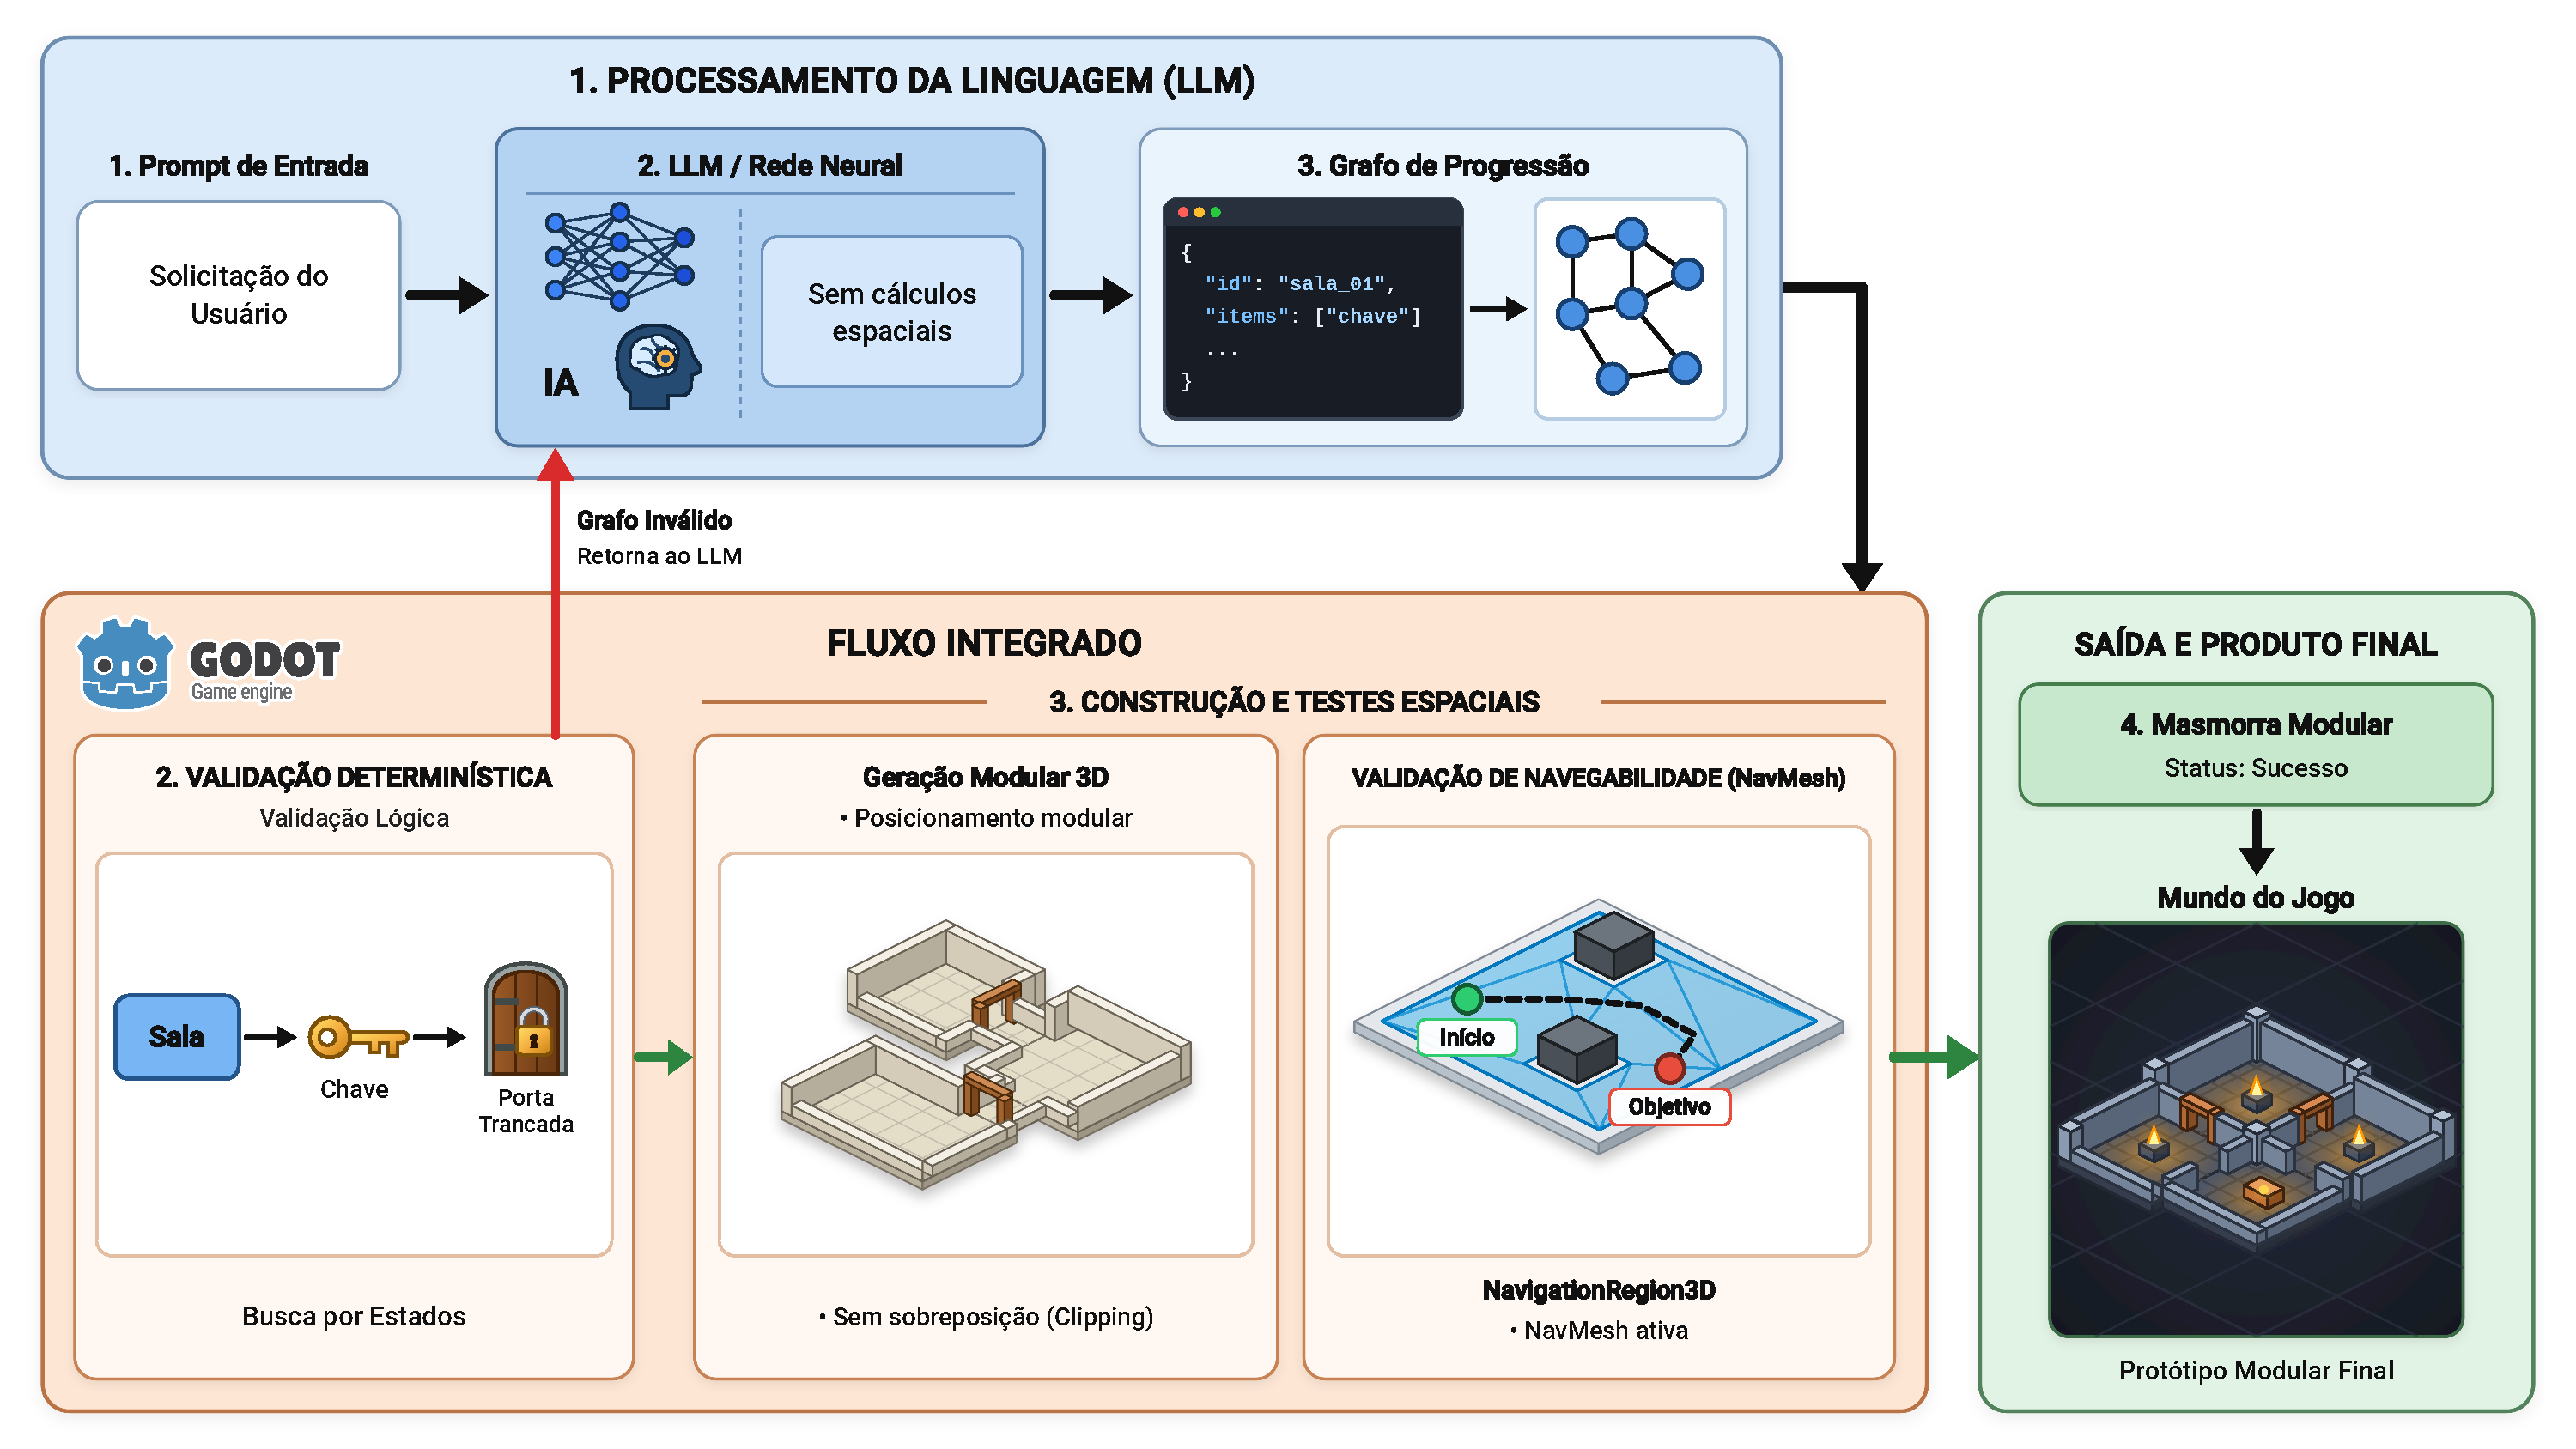
\includegraphics[width=0.95\linewidth]{diagrama_arquitetura_16x9}
  \captionof{figure}{Arquitetura híbrida proposta e fluxo integrado de geração e validação de fases 3D.}
\end{center}

%=============================================================================
% ◄ COLUNA DIREITA ►
%=============================================================================
\switchcolumn

\secao{Metodologia Experimental e Resultados Esperados}

{\fBody
Esta seção detalha os experimentos planejados para validar a arquitetura em desenvolvimento.

\vspace{3.5mm}
\noindent{\bfseries\itshape\color{sicverdescuro}Delineamento dos Experimentos}\par
\vspace{2mm}

Os experimentos gerarão amostras de fases (os parâmetros exatos para quantidade de prompts e repetições, faixas de salas, modelo/versão do LLM, temperatura, \textit{assets}, limites de tempo e tentativas serão fixados antes dos experimentos) sob dois tratamentos comparativos:

\begin{itemize}[leftmargin=16pt, itemsep=3pt, label={\color{sicverde}\faAngleRight}]
  \item \textbf{Grupo Controle:} LLM gera lógica e coordenadas 3D.
  \item \textbf{Grupo Experimental:} LLM gera o grafo de progressão e o módulo determinístico constrói e valida a geometria. Essa comparação avalia a arquitetura híbrida como um todo e não isola o efeito da validação.
\end{itemize}

Rotinas automatizadas auditarão como medida principal a proporção de fases que satisfazem simultaneamente as três classes de restrições; registrando-se também falhas de progressão, colisões, ausência de rota, tentativas e tempo total de geração (o tempo de construção da NavMesh será mantido apenas como medida auxiliar).

\vspace{3.5mm}
\noindent{\bfseries\itshape\color{sicverdescuro}Resultados Esperados}\par
\vspace{2mm}

\begin{itemize}[leftmargin=16pt, itemsep=3pt, label={\color{sicverde}\faAngleRight}]
  \item \textbf{Validade e Coerência das Fases:} A hipótese é que a arquitetura híbrida produza maior proporção de fases válidas e menor incidência de violações, hipótese que será testada experimentalmente.
  \item \textbf{Automatização:} Espera-se finalizar um \textit{plugin} no Godot convertendo linguagem natural em cenários editáveis diretamente no editor, otimizando o \textit{workflow} do artista técnico.
\end{itemize}
}\par

\divsec

\secao{Considera\c{c}\~{o}es Finais}

{\fBody
Este trabalho propõe superar deficiências dos LLMs no raciocínio espacial, transferindo cálculos à \textit{game engine}. A arquitetura e as regras estão em desenvolvimento. Os próximos passos serão implementar a conversão automática, verificar as restrições definidas e comparar as abordagens.
}\par

\divsec

\secao{Refer\^{e}ncias Bibliogr\'{a}ficas}

{\renewcommand*{\bibfont}{\fRef}%
\setlength{\bibitemsep}{4pt}%
\printbibliography[heading=none]}

\end{paracol}

% ===========================================================================
%  RODAPÉ GLOBAL ③ — linha verde + logo do evento + contato + QR Code
% ===========================================================================
\vspace{5mm}
{\color{sicverde}\rule{\linewidth}{2pt}}
\vspace{3mm}

% CORRIGIDO: texto do rodapé centralizado na largura total da folha.
\begin{center}
  {\fSmall\bfseries\color{sicverdescuro}
    XIII Semin\'{a}rio de Inicia\c{c}\~{a}o Cient\'{i}fica do IFNMG\\[3pt]
    24, 25 e 26 de novembro de 2026\enspace\textperiodcentered\enspace
    Campus Januária - MG
  }\\[4pt]
  {\fRef\color{siccinza}
    \faGlobe\enspace\url{www.ifnmg.edu.br}
    \quad\textbar\quad
    \faEnvelope\enspace\texttt{sic2026@ifnmg.edu.br}
  }
\end{center}

\end{document}
